\chapter{Passiv Radar Setup}
\section{Einführung}
\section{Hardware}
\subsection{ADALM-Pluto SDR}
Bei dem hier verwendeten SDR handelt es sich um ein ADALM
PLUTO SDR. Der Hauptgrund, warum sich in diesem Versuchsaufbau für dieses Gerät entschieden wurde ist die Bandbreite dieses Gerätes die bei bis zu 20 MHz liegt. Die Bandbreite des Signals was hier für Passiv Radar verwendet beträgt nämlich 5MHz was einige SDR nicht aufbringen können.  Aufs weitere besitzt das SDR eine Frequenz Abdeckung von 325 MHz bis zu 3.8 MHz. Die weiteren Daten können in der Tabelle abgelesen werden.

\subsubsection{Synchronität}
Zur Aufnahme des Referenzsignals als auch des reflektierten Signals werden jeweils ein Pluto-SDR benötigt, diese zwei müssen nun synchron betrieben werden. Dies wird erreicht durch Daisy Chaining  der beiden Uhren der SDRs und einer externen Uhr. Abbildung zeigt dann den fertigen Aufbau der Beiden SDRs und im Schaltplan in Abbildung ist zur erkennen wie die Uhr der jeweiligen SDRs aufgebaut ist.
\subsection{Antenne}
In diesem Aufbau werden zwei Antennen die für DVB-T gedacht sind verwendet. Die Antenne ist ein Yagi Antenne mit 43 Elementen wie man im Abbildung /ref{antenne} sieht die im Frequenzbereich von 470 bis 862 MHZ arbeitet, was für unseren Anwendungsfall sehr gut geeignet ist.Die weiteren Daten zur Antenne stehen in der Tabelle /ref{table:antenne}.

\begin{table}
    \centering
        \begin{tabular}[h]{rl}
            Antenne         & SKT SL43-01 UHF 43            \\
            Antennengewinn  & 11..13 dB                     \\
            Frequenzbereich & 470-862 MHz                   \\
            Halbwertsbreite & horiz. 30...40°/ver. 35...50° \\
        \end{tabular}
    \caption{Daten der SKT SL43-01 UHF 43 Antenne}\label{table:antenne}
\end{table}

\begin{figure}
    \centering
    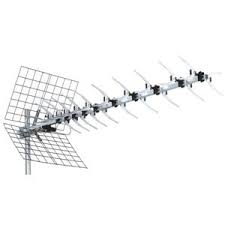
\includegraphics[width=\textwidth]{images/antenne.png}
    \caption{SKT SL43-01 UHF 43 Antenne}\label{antenne}
\end{figure}
\section{Signal}
\subsection{Aufbau von LTE}
\subsubsection{PSS}
\subsubsection{SSS}
\section{Software}
\subsection{SDR-angel}
\subsection{Signalverarbeitung}
\subsubsection{Ambiguity Funktion}
\subsubsection{Clean Algorithmus}
